\documentclass{article}
\usepackage[utf8]{inputenc}
\usepackage{graphicx}
\graphicspath{ {images/} }
\title{CS763 poisoning data}
\author{pierre.petrella, Miru Park }
\date{September 2019}

\begin{document}
\maketitle
\tableofcontents
\newpage
\section*{How secure are our classifiers? }
% ----------------- subsection---------------------
\subsection {potential threats of ML pipeline poisoning}
\paragraph{}
Machine learning systems have made itself necessary in this new data era requiring data analysis that can only be managed by automated processes. It is more precisely used for image recognition from distinguishing cats from dogs, red lights from green lights to facial recognition. 
\paragraph{}
Unfortunately these machine learning systems can be compromised. They are now becoming the weakest part of the security chain and consequently of the whole system. If no precautions are taken, this weakness can be used as a weapon by the attackers.

% ----------------- subsection---------------------
\subsection{General attack on a ML Pipeline}
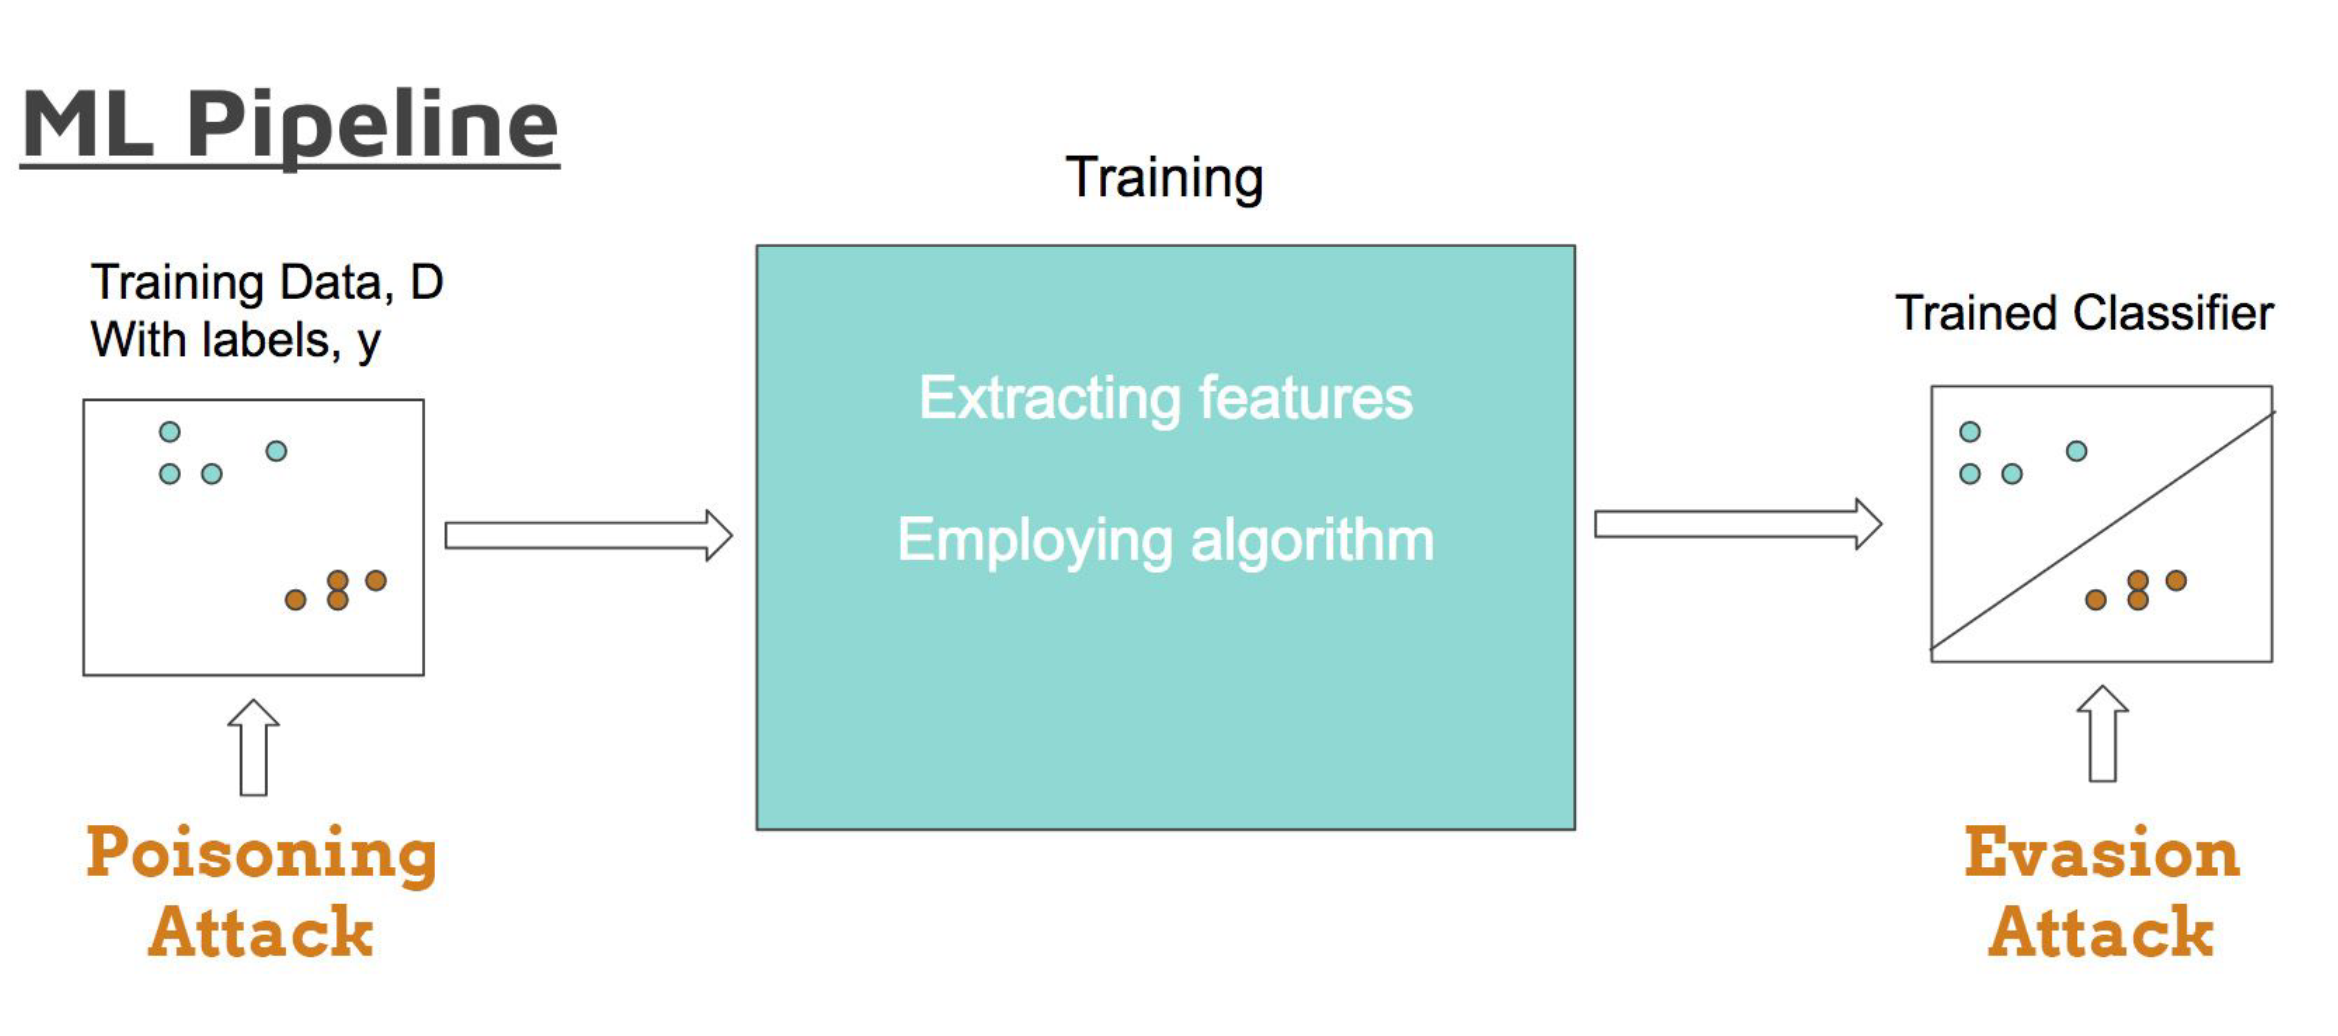
\includegraphics[scale=0.3]{MLpipeline.png}
% ----------------- section------------------------
\section{Targeted clean labor poisoning attacks on Neutral Networks}

% ----------------- subsection---------------------
\subsection{Properties}

The attacker has:
\begin{enumerate}
  \item No knowledge of the training data
  \item No control over the target instance during test time
  \item No control over labelling of data for training
  \item Knowledge of the model and it's parameters
\end{enumerate}
\paragraph{}
These restriction are quite strict on the attacker. This implies that the data poisoning requires minimal intrusion which makes it difficult to detect for the ML model.
% ----------------- subsection---------------------
\subsection{Properties}

\subsubsection*{Clean labels}
\paragraph{}
There are various types of poisoning attacks. In this paper, we are focusing on clean labels opposed to poisoning that involve tampering with the labels. clean labels allows to poison a training set with minimal intrusion as the poisoned image can simply be uploaded online and wait to be used by a ML model.

\subsubsection*{Targeted}
\paragraph{}
This type of attack is built to affect one image specifically and not tamper with the other ones. This allows the poisoning to happen without the Users noticing that the model was tampered with. the Degradation of the model should be unnoticeable.
\subsubsection*{good success rate}
\paragraph{}
If the poisoning is affecting the last more specific nodes of the ML model, we can assume that the poisoning will have a success rate of 100\% most of the time. 


% ----------------- subsection---------------------
\subsection{poisoning Attacks example}

\paragraph
We will be considering the Classifier that sorts between fish and dogs. The goal of the attacker will be to chose a specific picture of a fish and trick the ML model to think it is a dog. To do so he and insert a poisoned instance for fish class from dog a base instance. This poisoned picture which looks like a dog will be labeled accordingly and therefore trick the ML model.
\paragraph{}
Here are examples of poisoned dog images associated with the fish images they are targeting. We can see that the difference between the original and poisoned dog is indistinguishable to the human eye.   

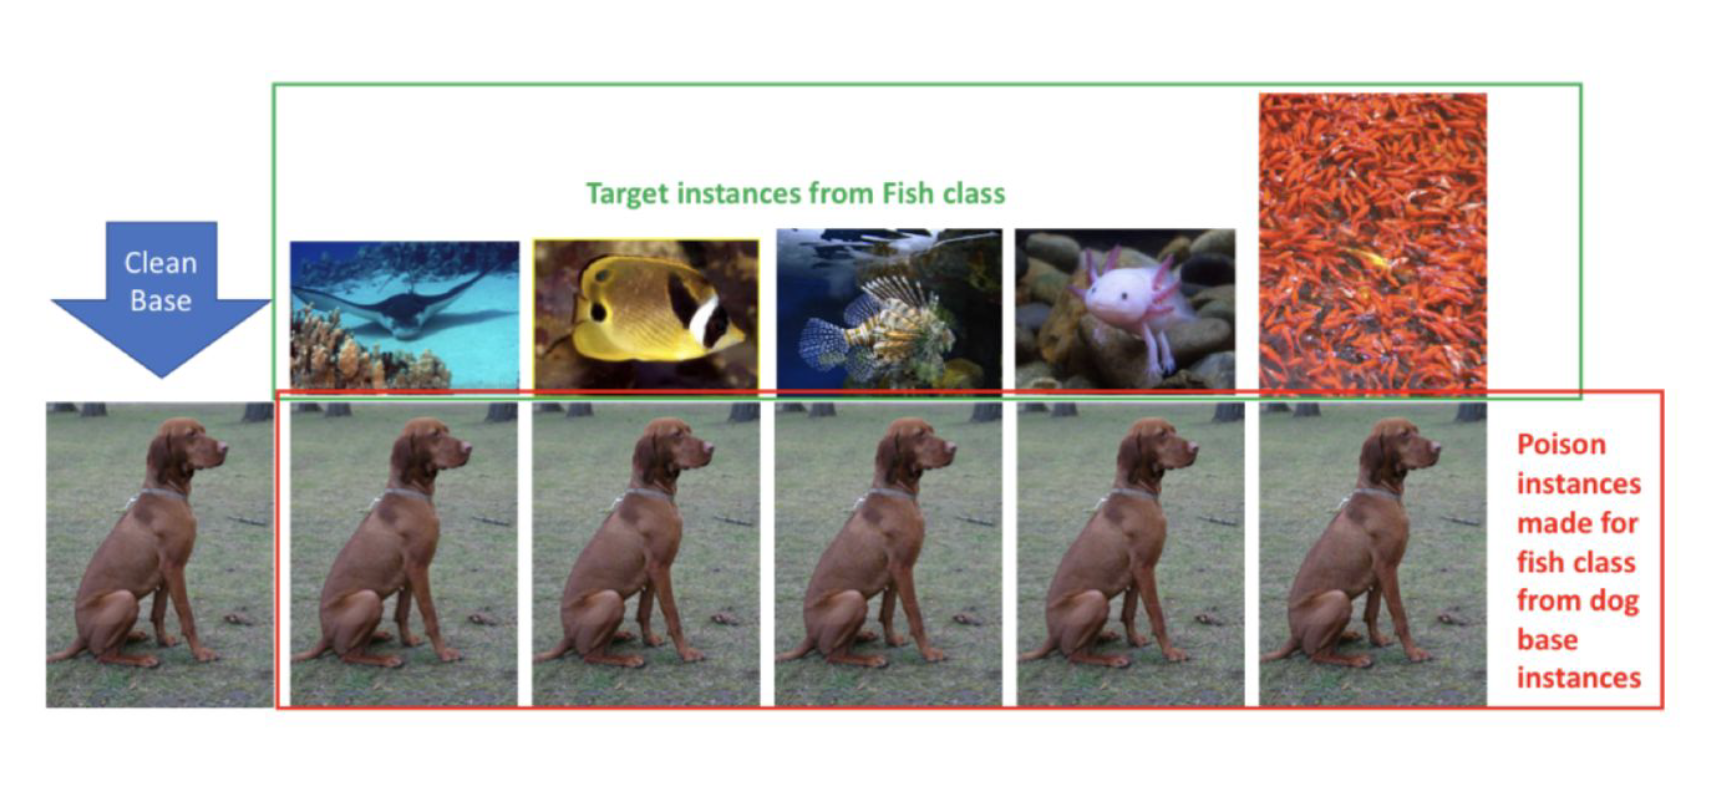
\includegraphics[scale=0.4]{ExamplePoisoning2.png}

% ----------------- subsection---------------------
\subsection{Transfer learning}
\paragraph{}
On way to train a new ML model is to use an existing working model that has been trained on a significantly big data set (Model A) and get rid of the last couple of layers. We then reconstruct the last layers using a relatively small data set to fine tune the model to distinguish cats and dogs for instance (Model B). 
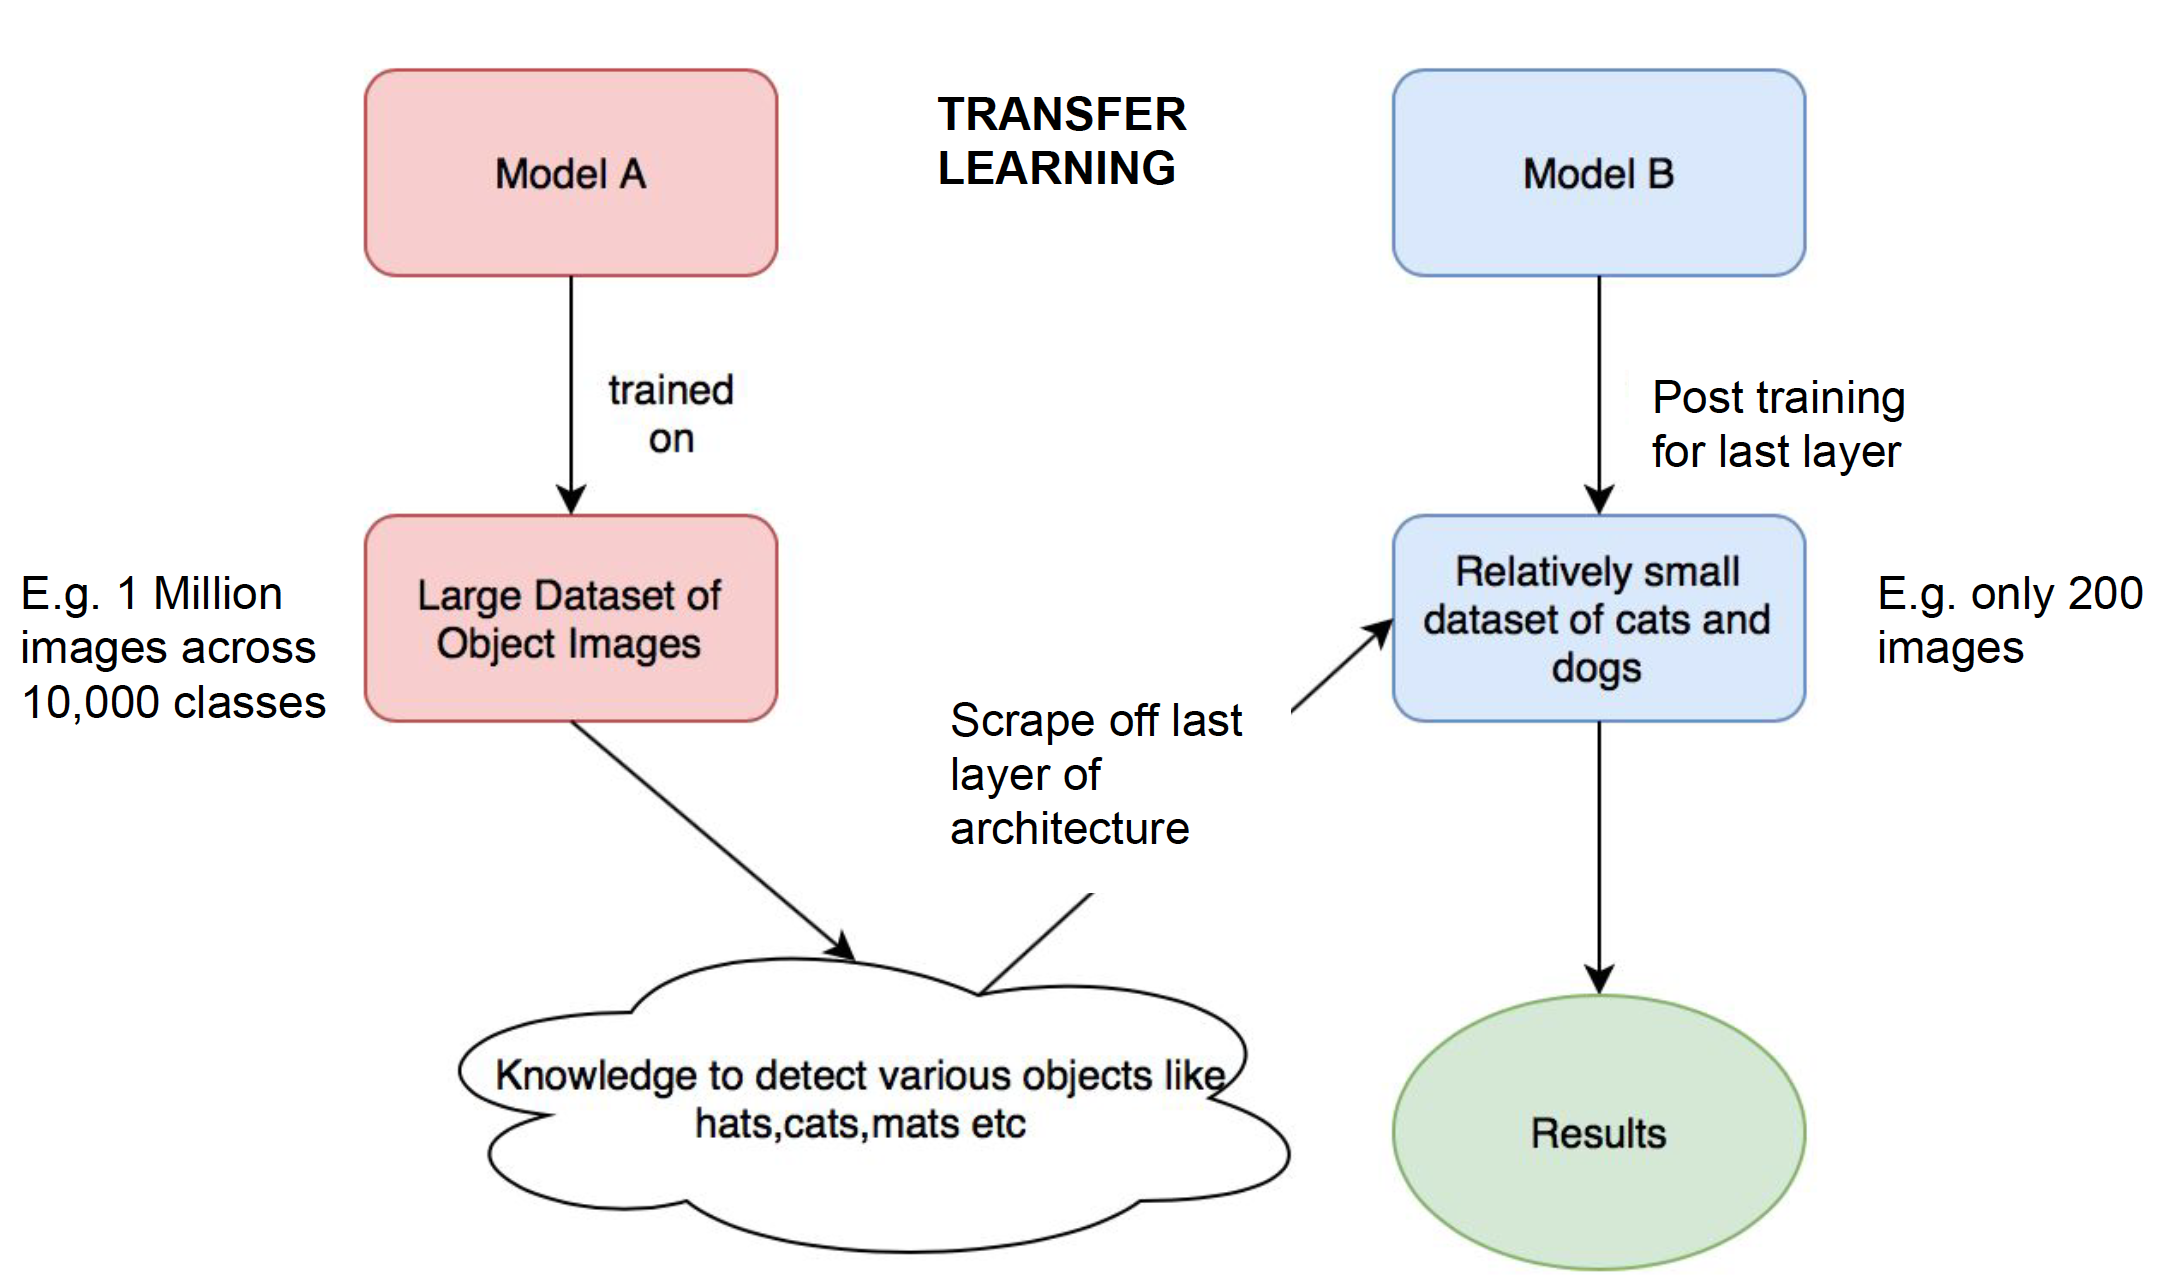
\includegraphics[scale=0.3]{MLTransfer.png}
\paragraph{}
These last layers are very susceptible to change making it an idea target for data poisoning. Transfer learning is an effective way to train a new model without requiring all the resources necessary to train a ML model from scratch. Unfortunately if the data set used to train the last layer has been tampered with classification accuracy can be easily tampered with. Here is another representation of Transfer learning. \\
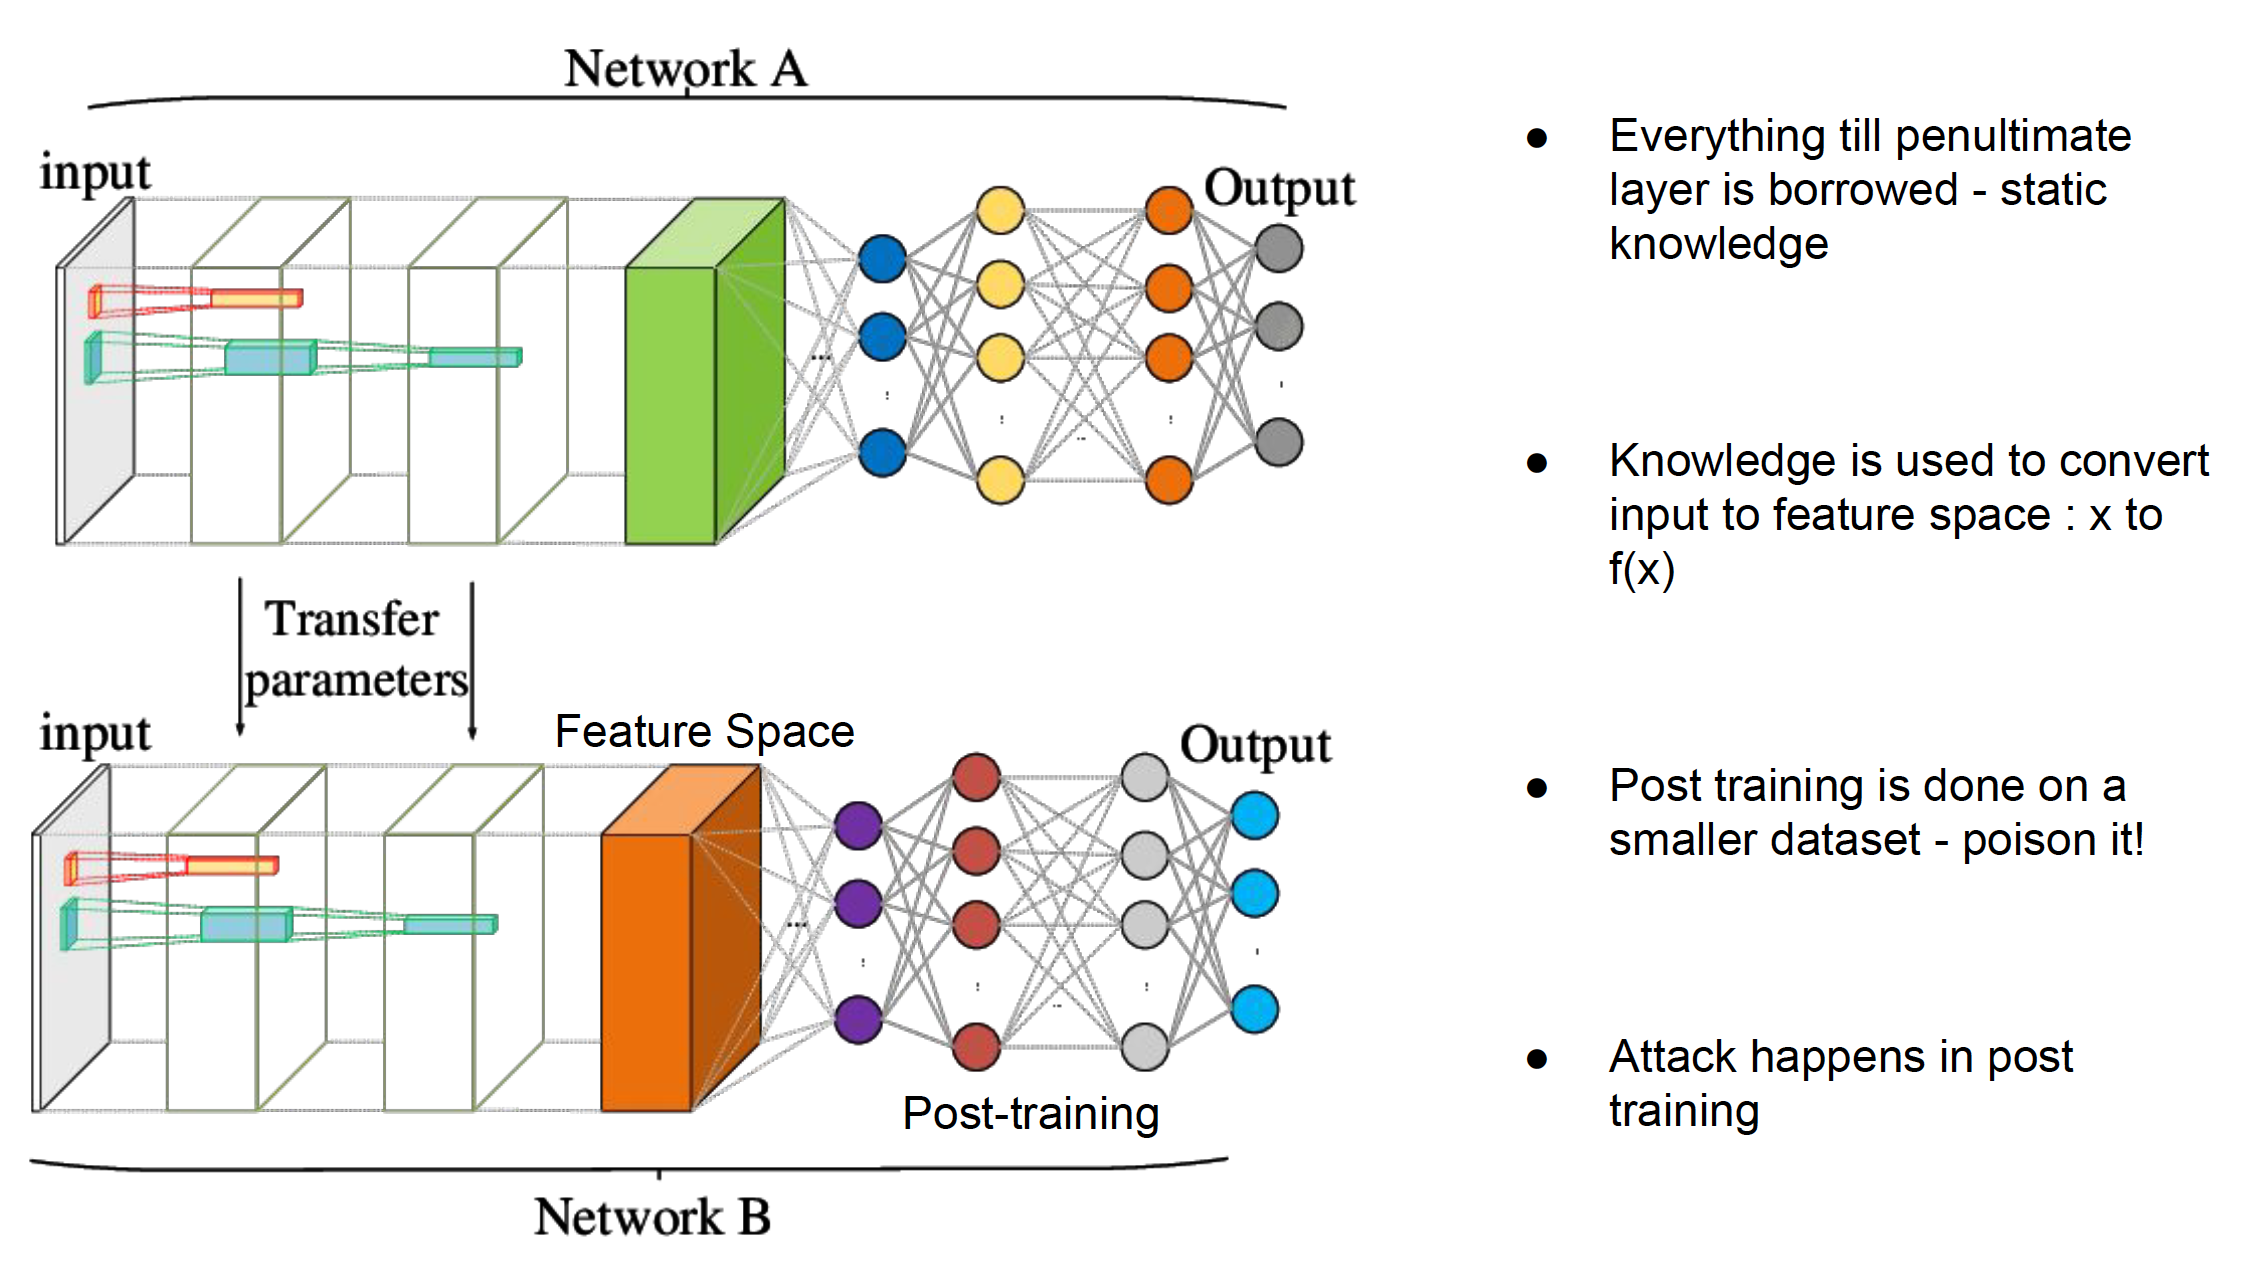
\includegraphics[scale=0.3]{MLTransfer2.png}

% ----------------- subsection---------------------
\subsection{Finding the poisoning}
\paragraph{}
The poisoning image must look like a dog but must have all the qualities of it's target (the fish). This will move the decision boundary from the initial doted line to the full line (see diagram). Now any pictures close enough to the targets characteristics will be on the "dog" side of the decision line and therefore be seen as a dog instead of a fish.

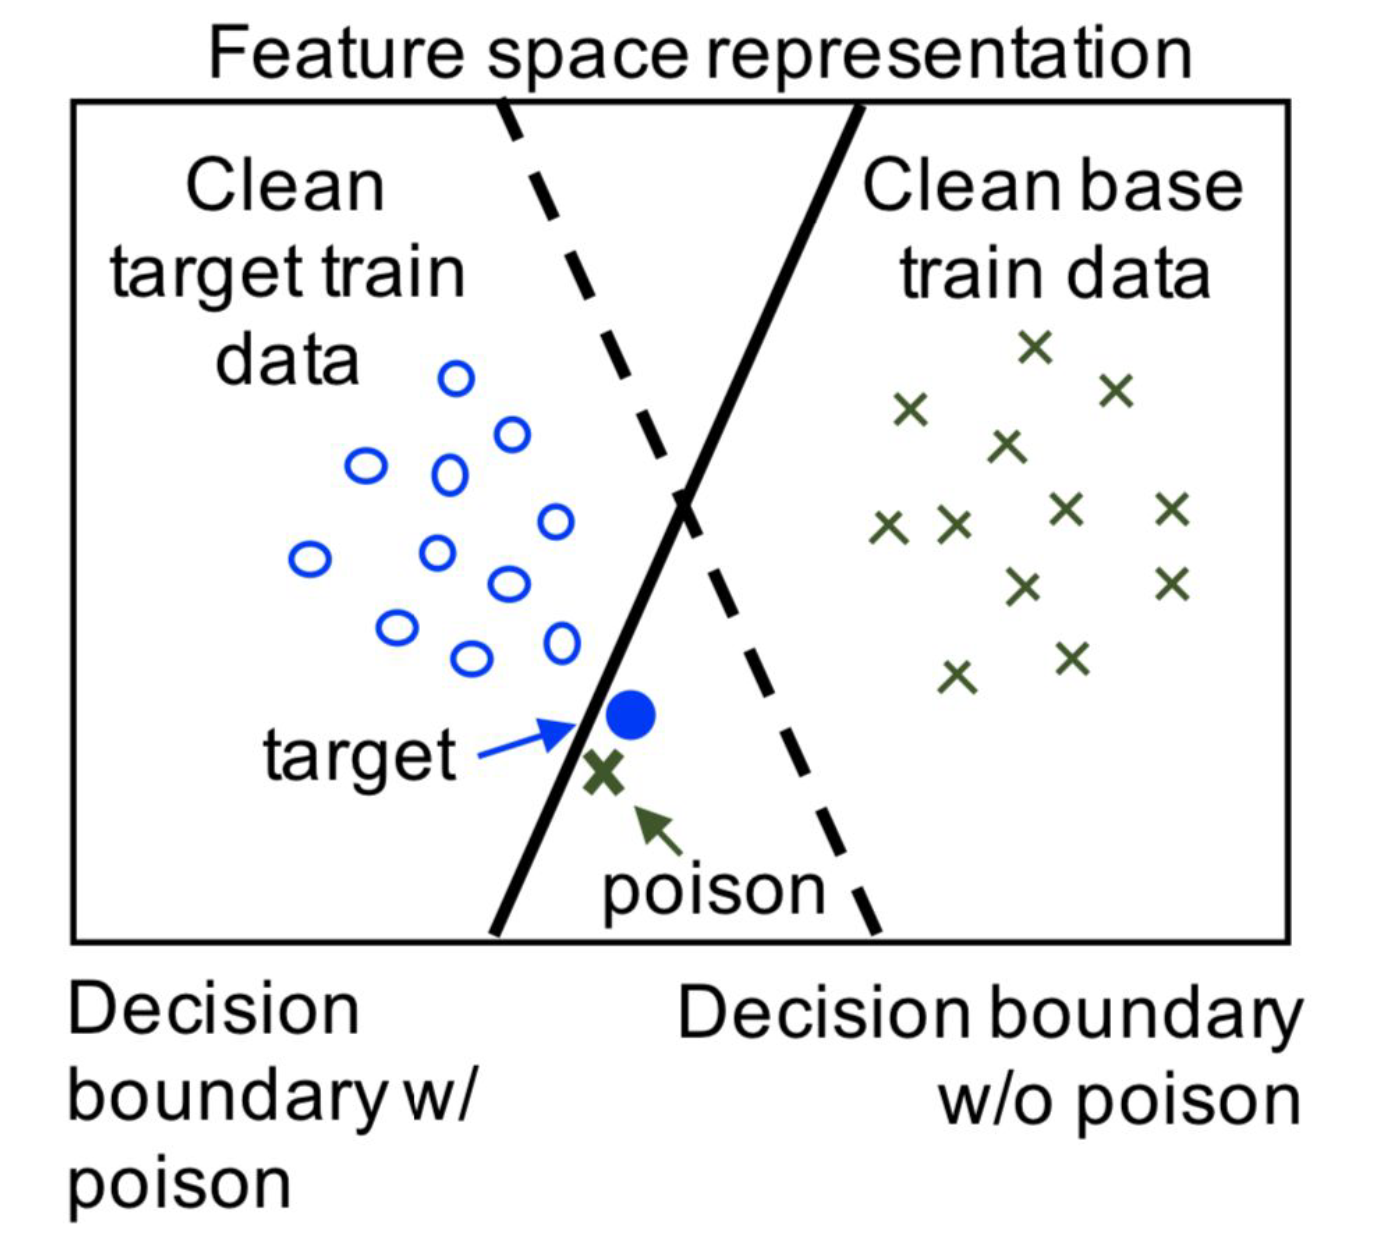
\includegraphics[scale=0.3]{DataLinePoison.png}
\paragraph{}
In order to create such a poisonous image we must find an image to satisfy this equation with X the image we want to find, t the target, b the initial "dog" image that we will modify and beta the importance we give to the similarity between the original a poisonous image: \\
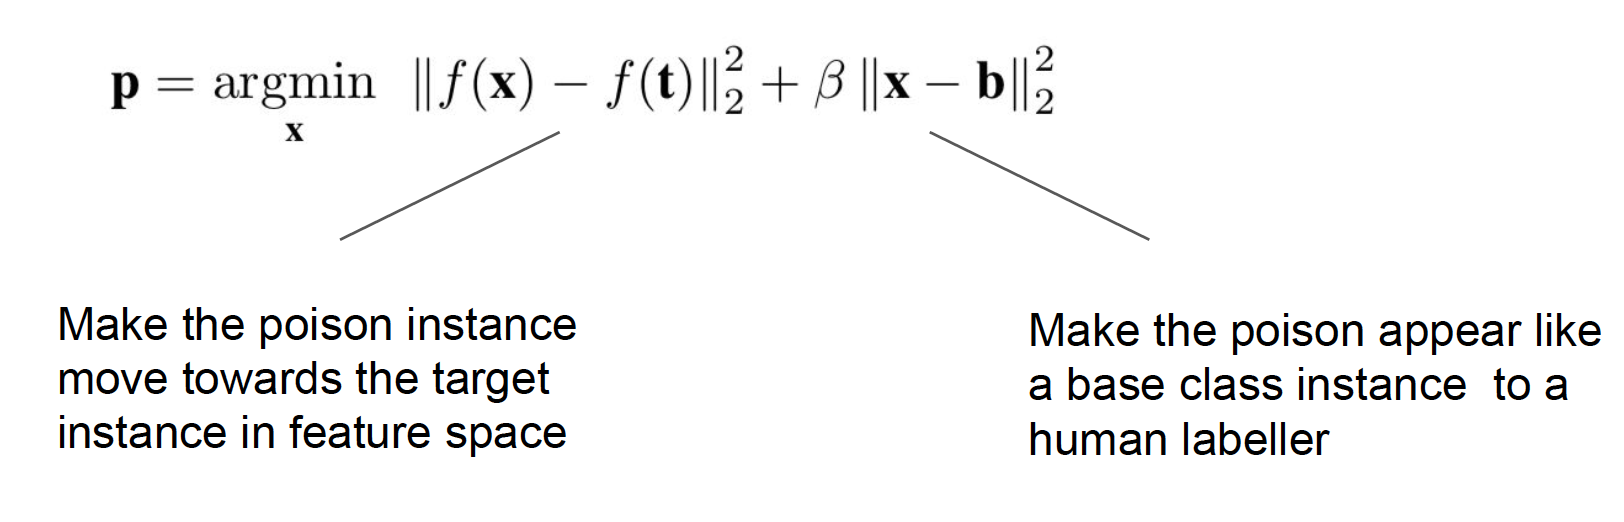
\includegraphics[scale=0.3]{Formula.png}

% ----------------- subsection---------------------
\subsection{Approach}
The protocol to follow to poison the data set is the following:

\begin{enumerate}
  \item Choose a target instance to misclassify
  \item Choose a base instance \& make imperceptible changes to it to get a poison
  \item Poison is created though an optimization based equation
  \item Inject poison into training data and let model be trained on poisoned dataset
\end{enumerate}

% ----------------- subsection---------------------
\subsection{Algorithm}
The algorithm to find the image consists of a forward backward iterative splitting procedure to find poison Iteratively. This is achieved by iterating these 2 steps:



\begin{enumerate}
  \item minimize distance to the target instance in feature space
  \item minimize distance from the base instance  in input space
\end{enumerate}

% ----------------- section------------------------
\section{What about Support Vector Machines (SVM)? Are they safe?}
\subsection {Overview of Data Poisoning Against SVM}
\paragraph{}
Poisoning attack against Support Vector Machines is an instance of causative attacks. Causative attack is an attack which takes advantage of many people's assumption that machine learning algorithms receive well-behaved data. However that is not so. An attacker that is sneaky enough can temper with optimal solutions to the Support Vector Machine by injecting a specific and well crafted attack example. Injection of such point into the training data is called Poisoning Attack.

\paragraph{}
Pictorially, the attacking scheme goes like this. $(x_c,y_c)$ is the desired attack point that will enable the attacker to temper with optimal solutions to the SVM and $D_{tr}$ is the training data$.

\paragraph{}
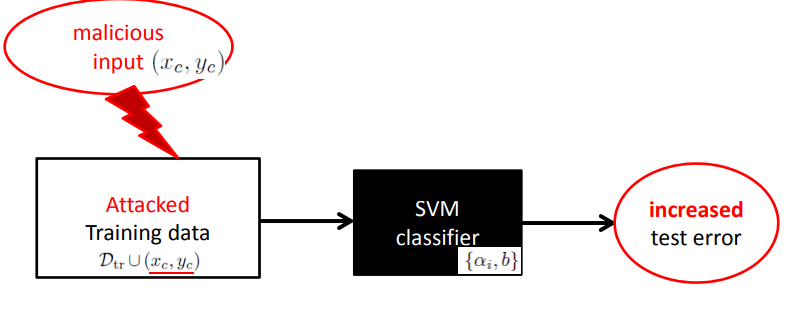
\includegraphics[scale=0.6]{poisoningpic.PNG}

\subsection {Brief overview of optimization}
\paragraph{}
Solving for optimal solutions to SVM can be achieved by mathematical optimization technique called quadratic programming. More precisely we solve a quadratic programming problem using Lagrange multipliers.
\paragraph{}
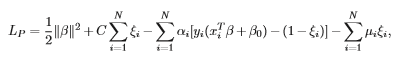
\includegraphics[scale=1.4]{LagrangePrimal.PNG}
Above equation is called the Lagrange Primal Function, abbreviated as $L_P$.
Upon minimizing the above function with respect to $\beta, \beta_0, \zeta_i \forall i$ we derive the following. 
\paragraph{}
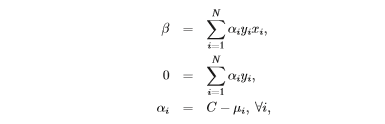
\includegraphics[scale=1.2]{PrimalConstraints.PNG}

\paragraph{}
Upon substitution of above variables back into our primal equation, we get the following:
\paragraph{}

\includegraphics[scale=1.2]{LagrangeDual.PNG}\\
\\
As suggested by the subscript D, we call this the Lagrange Dual Function.
\paragraph{}
Notice that now we have a function we can optimize with respect to only one variable, $\alpha$.
We optimize the Dual formulation of the Lagrangian subject to: $0 \leq \alpha_i \leq C$ and $\sum_{i=1}^{N}\alpha_iy_i$. There is however one more condition that needs to be satisfied and it is called the KKT. This condition gives us an extra set of three constraints that need to be satisfied on top of the ones we have seen so far. Here are the extra constraints that come from KKT:
\paragraph{}
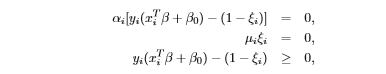
\includegraphics[scale=1.2]{KKTconsraints.PNG}
\paragraph{}
and keeping all these constraints in mind, we solve the dual formulation of the Lagrangian, substitute it back to the first constraint for the primal formulation of the Lagrangian and we get the solutions for the optimal weights:\\
\\
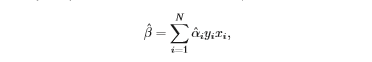
\includegraphics[scale=1.4]{dualprimalsolutions.PNG}\\
where of course, as can be seen in the original constrains, the coefficients are not zero.
\paragraph{}
Here is, more or less, a pictorial representation of what we described above.
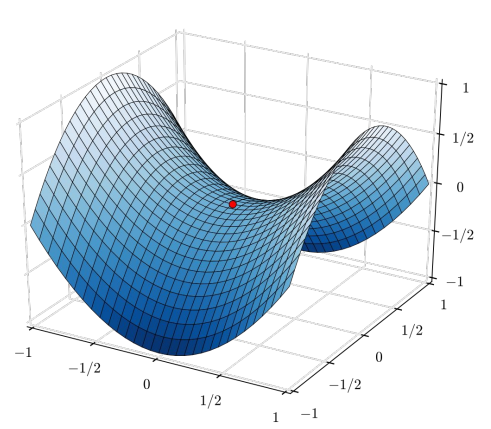
\includegraphics[scale=1]{optimizationPic.PNG}

\subsection{Refresher on SVM}
\paragraph{}
We assume that our data is linearly separable and our goal is to build a classifier (linear) to predict unobserved instances' labels.However, needless to say, this is an idea that comes from Perceptron. The goal of SVM is to find the "best" classifier. See below.
\paragraph{}

\includegraphics[scale=1.6]{bestseparation.PNG}
\\
\paragraph{}
It is clear from the picture which of the two linear boundaries is better. SVM's goal is to find such boundary. Thus more concretely, the goal is to maximize the margin $\rho$ and mathematically we come to the following formulation.
\paragraph{}
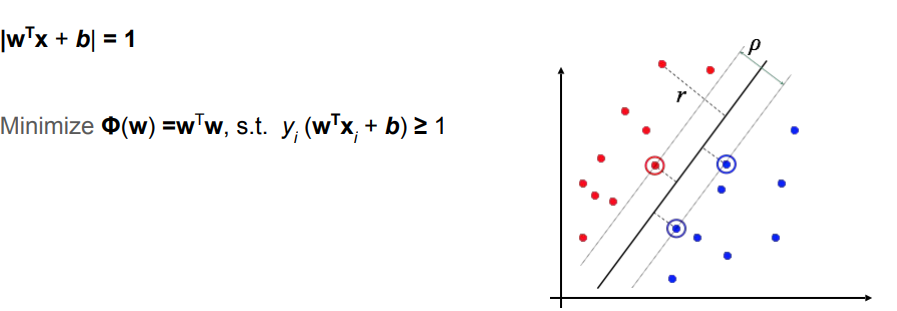
\includegraphics[scale=0.5]{bestmarginpic.PNG}
\\
\paragraph{}
However, we may not always guarantee that our data is perfectly linearly separable. In that case, we only need to slightly modify our formulation. Observe:\\
\paragraph{}
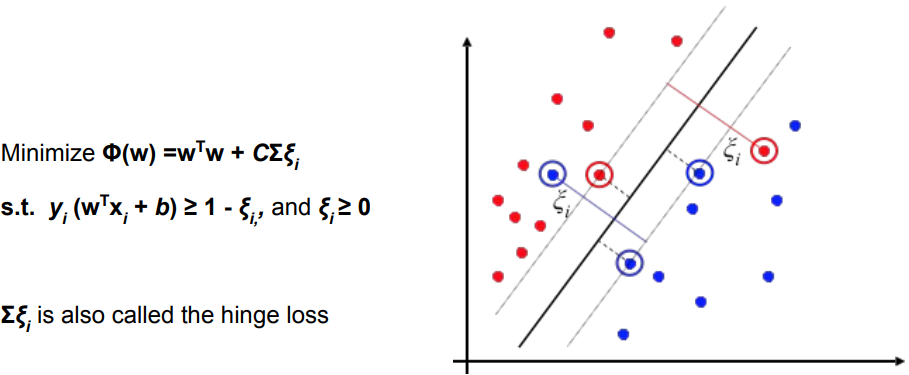
\includegraphics[scale=0.5]{bestmarginpic2.PNG}\\
\\
After some algebra, it is easy to see that $(W^{T}W^){-1}$ is the margin we wish to maximize with the slack variables $\zeta$. Above minimization problem can be translated to the quadratic formulation that was introduced earlier and optimal solutions can be derived in very much the same process illustrated above.
\subsection{Poisoning Attack}
So what can possibly go wrong? Quite a bit, as we will see from this point on. As mentioned in our earliest discussion of poisoning attacks, a sneaky and intelligent adversary can construct an instance that needs to only wait patiently until collection time of data for the training algorithm to rather maximize the hinge loss on the validation data. Such point can be found using the gradient ascent algorithm. The key is to update the attacking point with the addition of some appropriate gradient after each iteration. Thus, our problem is now to compute such gradient. This can also be formulated as a maximization problem: find $x_c$ such that the hinge loss function is maximized. The process of arriving to the solution is beyond the scope of this summary and one can study the referenced paper to see the derivation process. Nonetheless, we present the high-level idea of the algorithm.
\subsection{The Algorithm}
\begin{enumerate}
  \item Assumption: adversary knows the training data used by the learner and initial attack point is picked from a region sufficiently deep within the attacking class's ($y_c$ and this is arbitrary) margin
  \item input: Training Data, validation data, attack point label, initial attack point, step size, t
  \item output: $x_c$
  \item solve SVM on $D_tr$; compute $\{\alpha, b\}$
  \item pick initial attacking point $x_c^{0}$
  \item repeat until convergence (until the sequence of the Loss function satisfies the Cauchy-convergence criterion)
  \item perform gradient ascent 
\end{enumerate}

The high-level representation of gradient ascent is presented below
\paragraph{}
\begin{enumerate}
    \item recompute $\{\alpha, b\}$ on $D_{tr}$ U $\{x_c^{k}, y_c\}$
    \item compute the "poison" gradient u.
    \item normalize u
    \item $x_c^{k+1}$ = $x_c^{k} + tu$
\end{enumerate}

\paragraph{}
Here is the trajectory of the attacking point as the algorithm proceeds. 
\paragraph{}
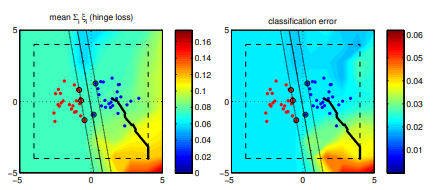
\includegraphics[scale=1]{poisontrajectory.PNG}
\subsection{Final Result}
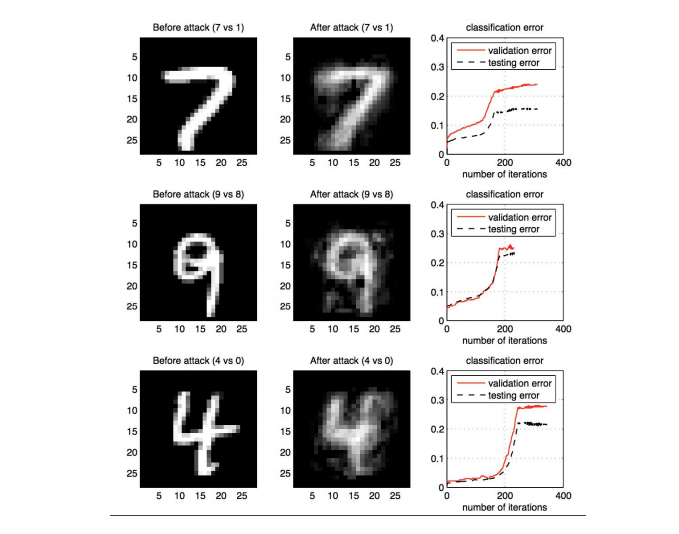
\includegraphics[scale=1]{finalResult.PNG}

\section*{Conclusion}
\end{document}